\section{Special linear transformations in $\R^2$}

\begin{outcome}
  \begin{enumerate}
  \item Find the matrix of rotations and reflections in $\R^2$ and
    determine the action of each on a vector in $\R^2$.
  \end{enumerate}
\end{outcome}

In this section, we will examine some special examples of linear transformations in $\R^2$ including rotations and reflections. We will use the geometric descriptions of vector addition and scalar
multiplication discussed earlier to show that a rotation of vectors through an angle and reflection of a vector across a line are examples of
linear transformations. 

More generally, denote a transformation given by a rotation by $T$. Why is such a transformation
linear? Consider the following picture which illustrates a rotation. Let $\vect{u},\vect{v}$ denote vectors. 

\begin{center}
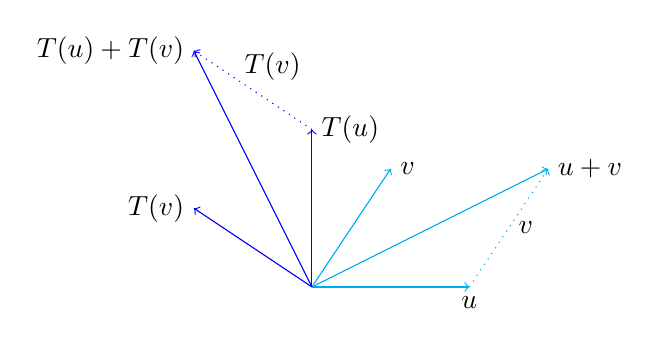
\begin{tikzpicture}
\draw[cyan, ->](0,0)--(2,0);
\draw[cyan,->](0,0)--(3,1.5);
\draw[cyan, ->](0,0)--(1,1.5);
\draw[cyan, dotted, ->](2,0)--(3,1.5);
\draw[blue, ->](0,0)--(0,2);
\draw[blue, ->](0,0)--(-1.5, 3);
\draw[blue, ->](0,0)--(-1.5,1);
\draw[blue, dotted, ->](0,2)--(-1.5,3);
\node[below] at (2,0){$\vect{u}$};
\node[right] at (2.5,0.75){$\vect{v}$};
\node[right] at (3,1.5){$\vect{u}+\vect{v}$};
\node[right] at (1,1.5){$\vect{v}$};
\node[right] at (0,2){$T(\vect{u})$};
\node[left] at (-1.5,3){$T(\vect{u})+T(\vect{v})$};
\node[left] at (-1.5,1){$T(\vect{v})$};
\node[above] at (-0.5,2.5){$T(\vect{v})$};
\end{tikzpicture}
\end{center}

Let's consider how to obtain $T\tup{\vect{u}+\vect{v}}$. 
Simply, you add $T (\vect{u})$ and $T(\vect{v})$. 
Here is why. If you add $T(\vect{u})$ to $T(\vect{v})$ you get
the diagonal of the parallelogram determined by $T(\vect{u})$ and $T(\vect{v})$, as this action
is our usual vector addition.
Now, suppose we first add $\vect{u}$ and $\vect{v}$, and then apply the transformation $T$ to 
$\vect{u}+\vect{v}$. Hence, we find $T( \vect{u}+\vect{v})$. 
As shown in the diagram, this will result in the same vector. In other words, $T(\vect{u}+\vect{v}) = T(\vect{u}) 
+ T(\vect{v})$. 

This is because the rotation preserves all angles between the vectors
as well as their lengths. In particular, it preserves the shape of
this parallelogram. Thus both
$T\tup{\vect{u}}+T\tup{\vect{v}}$ and
$T\tup{\vect{u}+\vect{v}}$ give the same vector. It follows
that $T$ distributes across addition of the vectors of
$\R^{2}$.

Similarly, if $k$ is a scalar, it follows that $T\tup{k\vect{u}}=kT\tup{\vect{u}}$.
Thus rotations are an example of a
linear transformation by Definition \ref{def:linear-transformation}.

The following theorem gives the matrix of a linear transformation which rotates all vectors through an angle of $\theta$. 

\begin{theorem}{Rotation}{rotation}
Let $R_{\theta}: \R^2 \to \R^2$ be a linear transformation given by rotating vectors through an angle of $\theta$. Then the matrix $A$ of $R_{\theta}$ is given by 
\[
\begin{mymatrix}{rr}
\cos \tup{\theta } & -\sin \tup{\theta } \\
\sin \tup{\theta } & \cos \tup{\theta }
\end{mymatrix}
\]
\end{theorem}

\begin{proof}
Let $\vect{e}_{1} = \begin{mymatrix}{r}
1 \\
0
\end{mymatrix} $ and $\vect{e}_{2} = \begin{mymatrix}{r}
0 \\
1
\end{mymatrix}$. These identify the geometric vectors which point along the
positive $x$ axis and positive $y$ axis as shown.

\begin{center}
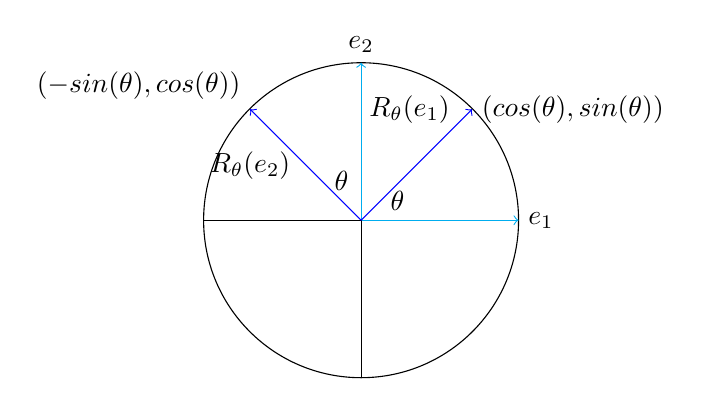
\begin{tikzpicture}
\draw(0,0) circle [radius=2];
\draw(-2,0)--(0,0);
\draw[cyan, ->](0,0)--(2,0);
\draw(0,-2)--(0,0);
\draw[cyan,->](0,0)--(0,2);
\draw[blue, ->](0,0)--(1.41,1.41);
\draw[blue, ->](0,0)--(-1.41,1.41);
\node[right] at (2,0){$\vect{e}_1$};
\node[above] at (0,2){$\vect{e}_2$};
\node[left] at (1.25,1.41){$R_{\theta}(\vect{e}_1)$};
\node[below] at (-1.41,1){$R_{\theta}(\vect{e}_2)$};
\node[right] at (1.41,1.41){$(cos(\theta), sin(\theta))$};
\node[above left] at (-1.41,1.41){$(-sin(\theta), cos(\theta))$};
\node[right] at (0.25,0.25){$\theta$};
\node[above] at (-0.25,0.25){$\theta$};
\end{tikzpicture}
\end{center}
 
From Theorem \ref{thm:matrix-of-linear-transformation}, we need to find $R_{\theta}(\vect{e}_{1})$ and $R_{\theta}(\vect{e}_{2}), $
and use these as the columns of the matrix $A$ of $T$. We can use  
$\func{cos},\func{sin}$ of the angle $\theta$ to find the coordinates of $R_{\theta}(\vect{e}_{1})$ as shown
in the above picture. The coordinates of $R_{\theta}(\vect{e}_{2})$ also follow from
trigonometry. Thus
\begin{equation*}
R_{\theta}(\vect{e}_{1})=\begin{mymatrix}{r}
\cos \theta \\
\sin \theta
\end{mymatrix} ,R_{\theta}(\vect{e}_{2})=\begin{mymatrix}{r}
-\sin \theta \\
\cos \theta
\end{mymatrix} 
\end{equation*}
Therefore, from Theorem \ref{thm:matrix-of-linear-transformation},
\begin{equation*}
A=\begin{mymatrix}{rr}
\cos \theta & -\sin \theta \\
\sin \theta & \cos \theta
\end{mymatrix}
\end{equation*}

We can also prove this algebraically without the use of the
above picture. The definition of $\tup{
\cos \tup{\theta } ,\sin \tup{\theta } } $ is as the 
coordinates of the point of $R_{\theta}(\vect{e}_{1})$.  Now the point of
the vector $\vect{e}_{2}$ is exactly $\pi /2$ further along the unit circle from 
the point of $\vect{e}_{1}$, and therefore after rotation through an angle of $\theta $ the coordinates
$x$ and $y$ of the point of $R_{\theta}(\vect{e}_{2})$ are given by
\begin{equation*}
\tup{x,y} =\tup{\cos \tup{\theta +\pi /2} ,\sin \tup{
\theta +\pi /2} } =\tup{-\sin \theta ,\cos \theta } 
\end{equation*}

\end{proof}

Consider the following example. 

\begin{example}{Rotation in $\R^2$}{rotation}
Let $R_{\frac{\pi}{2}}: \R^2 \to \R^2$ denote rotation through $\pi/2$. Find the matrix of $R_{\frac{\pi}{2}}$. Then, find $R_{\frac{\pi}{2}} (\vect{x})$ where $\vect{x} = \begin{mymatrix}{r}
1 \\
-2
\end{mymatrix}$. 
\end{example}

\begin{solution}
By Theorem \ref{thm:rotation}, the matrix of $R_{\frac{\pi}{2}}$ is given by
\[
\begin{mymatrix}{rr}
\cos \tup{\theta } & -\sin \tup{\theta } \\
\sin \tup{\theta } & \cos \tup{\theta }
\end{mymatrix}
=
\begin{mymatrix}{rr}
\cos \tup{\pi/2 } & -\sin \tup{\pi/2 } \\
\sin \tup{\pi/2 } & \cos \tup{\pi/2 }
\end{mymatrix}
=
\begin{mymatrix}{rr}
0 & -1 \\
1 & 0 
\end{mymatrix}
\]

To find $R_{\frac{\pi}{2}} (\vect{x})$, we multiply the matrix of $R_{\frac{\pi}{2}}$ by $\vect{x}$ as follows
\[
\begin{mymatrix}{rr}
0 & -1 \\
1 & 0 
\end{mymatrix}
\begin{mymatrix}{r}
1 \\
-2 
\end{mymatrix}
=
\begin{mymatrix}{r}
2 \\
1
\end{mymatrix}
\]

\end{solution}

We now look at an example of a linear transformation involving two angles.

\begin{example}{The rotation matrix of the sum of two angles}{rotation-matrix-two-angles}
Find the matrix of the linear transformation which is
obtained by first rotating all vectors through an angle of $\phi $ and then
through an angle $\theta$. Hence the linear transformation 
rotates all vectors through an angle of $\theta +\phi $.
\end{example}

\begin{solution}
Let $R_{\theta +\phi }$ denote the linear transformation which rotates every
vector through an angle of $\theta +\phi$. 
Then to obtain $R_{\theta +\phi }$,
we first apply $R_{\phi }$ and then $R_{\theta }$ where $R_{\phi }$
is the linear transformation which rotates through an angle of $\phi $ and 
$R_{\theta }$ is the linear transformation which rotates through an angle of 
$\theta$. Denoting the corresponding matrices by $A_{\theta +\phi }$, 
$A_{\phi }$, and $A_{\theta }$, it follows that for every $\vect{u}$
\begin{equation*}
R_{\theta +\phi }\tup{\vect{u}}=A_{\theta +\phi }\vect{u}=A_{\theta }A_{\phi }\vect{u} = R_{\theta }R_{\phi }
\tup{\vect{u}}
\end{equation*}
Notice the order of the matrices here! 

Consequently, you must have
\begin{eqnarray*}
A_{\theta +\phi } &=&\begin{mymatrix}{cc}
\cos \tup{\theta +\phi } & -\sin \tup{\theta +\phi } \\
\sin \tup{\theta +\phi } & \cos \tup{\theta +\phi }
\end{mymatrix}\\
&=&\begin{mymatrix}{cc}
\cos \theta & -\sin \theta \\
\sin \theta & \cos \theta
\end{mymatrix} \begin{mymatrix}{cc}
\cos \phi & -\sin \phi \\
\sin \phi & \cos \phi
\end{mymatrix} 
 =A_{\theta }A_{\phi } 
\end{eqnarray*}

The usual matrix multiplication 
yields
\begin{eqnarray*}
A_{\theta +\phi } &=& \begin{mymatrix}{cc}
\cos \tup{\theta +\phi } & -\sin \tup{\theta +\phi } \\
\sin \tup{\theta +\phi } & \cos \tup{\theta +\phi }
\end{mymatrix} \\
&=&\begin{mymatrix}{cc}
\cos \theta \cos \phi -\sin \theta \sin \phi & -\cos \theta \sin \phi -\sin
\theta \cos \phi \\
\sin \theta \cos \phi +\cos \theta \sin \phi & \cos \theta \cos \phi -\sin
\theta \sin \phi
\end{mymatrix} \\
&=& A_{\theta }A_{\phi } 
\end{eqnarray*}

Don't these look familiar? They are the usual trigonometric identities for the sum
of two angles derived here using linear algebra concepts.
\index{trigonometry!sum of two angles}

\end{solution}

Here we have focused on rotations in two dimensions. However, you can consider rotations and
other geometric concepts in any number of dimensions. This is one of the
major advantages of linear algebra. You can break down a difficult
geometrical procedure into small steps, each corresponding to multiplication
by an appropriate matrix. Then by multiplying the matrices, you can obtain a
single matrix which can give you numerical information on the results of
applying the given sequence of simple procedures.


Linear transformations which reflect vectors across a line are a second important type of transformations in $\R^2$. Consider the following theorem.

\begin{theorem}{Reflection}{reflection}
Let $Q_m: \R^2 \to \R^2$ be a linear transformation given by reflecting vectors over the line $\vect{y}=m\vect{x}$. Then the matrix of $Q_m$ is given by 
\[
\frac{1}{1+m^2}
\begin{mymatrix}{cc}
1-m^2 & 2m \\
2m & m^2-1 
\end{mymatrix}
\]
\end{theorem}

Consider the following example. 

\begin{example}{Reflection in $\R^2$}{reflection}
Let $Q_2: \R^2 \to \R^2$ denote reflection over the line $\vect{y}=2\vect{x}$. Then $Q_2$ is a linear transformation. Find the matrix of $Q_2$. Then, find $Q_2 (\vect{x})$ where $\vect{x} = \begin{mymatrix}{r}
1 \\
-2
\end{mymatrix}$. 
\end{example}

\begin{solution}
By Theorem \ref{thm:reflection}, the matrix of $Q_2$ is given by 
\[
\frac{1}{1+m^2}
\begin{mymatrix}{cc}
1-m^2 & 2m \\
2m & m^2-1 
\end{mymatrix}
=
\frac{1}{1+(2)^2}
\begin{mymatrix}{cc}
1-(2)^2 & 2(2) \\
2(2) & (2)^2-1 
\end{mymatrix}
=
\frac{1}{5}
\begin{mymatrix}{rr}
-3 & 8 \\
8 & 3 
\end{mymatrix}
\]

To find $Q_2(\vect{x})$ we multiply $\vect{x}$ by the matrix of $Q_2$ as follows:
\[
\frac{1}{5}
\begin{mymatrix}{rr}
-3 & 8 \\
8 & 3 
\end{mymatrix}
\begin{mymatrix}{r}
1 \\
-2
\end{mymatrix}
=
\begin{mymatrix}{r}
-\vspace{0.05in}\frac{19}{5} \\
\vspace{0.05in}\frac{2}{5}
\end{mymatrix}
\]

\end{solution}

Consider the following example which incorporates a reflection as well as a rotation of vectors.

\begin{example}{Rotation followed by a reflection}{rotation-reflection}
Find the matrix of the linear transformation which is obtained by first
rotating all vectors through an angle of $\pi /6$ and then reflecting
through the $x$ axis.
\end{example}

\begin{solution}
By Theorem \ref{thm:rotation}, the matrix of the transformation which
involves rotating through an angle of $\pi /6$ is
\begin{equation*}
\begin{mymatrix}{rr}
\cos \tup{\pi /6} & -\sin \tup{\pi /6} \\
\sin \tup{\pi /6} & \cos \tup{\pi /6}
\end{mymatrix} =\begin{mymatrix}{cc}
\vspace{0.05in}\frac{1}{2}\sqrt{3} & -\vspace{0.05in}\frac{1}{2} \\
\vspace{0.05in}\frac{1}{2} & \vspace{0.05in}\frac{1}{2}\sqrt{3}
\end{mymatrix}
\end{equation*}

Reflecting across the $x$ axis is the same action as reflecting vectors over the line $\vect{y}=m\vect{x}$ with $m=0$. By Theorem \ref{thm:reflection}, the matrix for the transformation which reflects all vectors through the $x$
axis is
\begin{equation*}
\frac{1}{1+m^2}
\begin{mymatrix}{cc}
1-m^2 & 2m \\
2m & m^2-1 
\end{mymatrix}
=
\frac{1}{1+(0)^2}
\begin{mymatrix}{cc}
1-(0)^2 & 2(0) \\
2(0) & (0)^2-1 
\end{mymatrix}
=
\begin{mymatrix}{rr}
1 & 0 \\
0 & -1
\end{mymatrix} 
\end{equation*}

Therefore, the matrix of the linear transformation which first rotates
through $\pi /6$ and then reflects through the $x$ axis is given by 
\begin{equation*}
\begin{mymatrix}{rr}
1 & 0 \\
0 & -1
\end{mymatrix} \begin{mymatrix}{rr}
\vspace{0.05in}\frac{1}{2}\sqrt{3} & -\vspace{0.05in}\frac{1}{2} \\
\vspace{0.05in}\frac{1}{2} & \vspace{0.05in}\frac{1}{2}\sqrt{3}
\end{mymatrix} =\allowbreak \begin{mymatrix}{rr}
\vspace{0.05in}\frac{1}{2}\sqrt{3} & -\vspace{0.05in}\frac{1}{2} \\
-\vspace{0.05in}\frac{1}{2} & -\vspace{0.05in}\frac{1}{2}\sqrt{3}
\end{mymatrix} 
\end{equation*}
\end{solution}
